% Options for packages loaded elsewhere
\PassOptionsToPackage{unicode}{hyperref}
\PassOptionsToPackage{hyphens}{url}
%
\documentclass[
]{article}
\usepackage{lmodern}
\usepackage{amssymb,amsmath}
\usepackage{ifxetex,ifluatex}
\ifnum 0\ifxetex 1\fi\ifluatex 1\fi=0 % if pdftex
  \usepackage[T1]{fontenc}
  \usepackage[utf8]{inputenc}
  \usepackage{textcomp} % provide euro and other symbols
\else % if luatex or xetex
  \usepackage{unicode-math}
  \defaultfontfeatures{Scale=MatchLowercase}
  \defaultfontfeatures[\rmfamily]{Ligatures=TeX,Scale=1}
\fi
% Use upquote if available, for straight quotes in verbatim environments
\IfFileExists{upquote.sty}{\usepackage{upquote}}{}
\IfFileExists{microtype.sty}{% use microtype if available
  \usepackage[]{microtype}
  \UseMicrotypeSet[protrusion]{basicmath} % disable protrusion for tt fonts
}{}
\makeatletter
\@ifundefined{KOMAClassName}{% if non-KOMA class
  \IfFileExists{parskip.sty}{%
    \usepackage{parskip}
  }{% else
    \setlength{\parindent}{0pt}
    \setlength{\parskip}{6pt plus 2pt minus 1pt}}
}{% if KOMA class
  \KOMAoptions{parskip=half}}
\makeatother
\usepackage{xcolor}
\IfFileExists{xurl.sty}{\usepackage{xurl}}{} % add URL line breaks if available
\IfFileExists{bookmark.sty}{\usepackage{bookmark}}{\usepackage{hyperref}}
\hypersetup{
  pdftitle={Parce que c'est votre projet, utilisez RStudio !},
  pdfauthor={Camille Magneville \& Gaël Mariani},
  hidelinks,
  pdfcreator={LaTeX via pandoc}}
\urlstyle{same} % disable monospaced font for URLs
\usepackage[margin=1in]{geometry}
\usepackage{color}
\usepackage{fancyvrb}
\newcommand{\VerbBar}{|}
\newcommand{\VERB}{\Verb[commandchars=\\\{\}]}
\DefineVerbatimEnvironment{Highlighting}{Verbatim}{commandchars=\\\{\}}
% Add ',fontsize=\small' for more characters per line
\usepackage{framed}
\definecolor{shadecolor}{RGB}{248,248,248}
\newenvironment{Shaded}{\begin{snugshade}}{\end{snugshade}}
\newcommand{\AlertTok}[1]{\textcolor[rgb]{0.94,0.16,0.16}{#1}}
\newcommand{\AnnotationTok}[1]{\textcolor[rgb]{0.56,0.35,0.01}{\textbf{\textit{#1}}}}
\newcommand{\AttributeTok}[1]{\textcolor[rgb]{0.77,0.63,0.00}{#1}}
\newcommand{\BaseNTok}[1]{\textcolor[rgb]{0.00,0.00,0.81}{#1}}
\newcommand{\BuiltInTok}[1]{#1}
\newcommand{\CharTok}[1]{\textcolor[rgb]{0.31,0.60,0.02}{#1}}
\newcommand{\CommentTok}[1]{\textcolor[rgb]{0.56,0.35,0.01}{\textit{#1}}}
\newcommand{\CommentVarTok}[1]{\textcolor[rgb]{0.56,0.35,0.01}{\textbf{\textit{#1}}}}
\newcommand{\ConstantTok}[1]{\textcolor[rgb]{0.00,0.00,0.00}{#1}}
\newcommand{\ControlFlowTok}[1]{\textcolor[rgb]{0.13,0.29,0.53}{\textbf{#1}}}
\newcommand{\DataTypeTok}[1]{\textcolor[rgb]{0.13,0.29,0.53}{#1}}
\newcommand{\DecValTok}[1]{\textcolor[rgb]{0.00,0.00,0.81}{#1}}
\newcommand{\DocumentationTok}[1]{\textcolor[rgb]{0.56,0.35,0.01}{\textbf{\textit{#1}}}}
\newcommand{\ErrorTok}[1]{\textcolor[rgb]{0.64,0.00,0.00}{\textbf{#1}}}
\newcommand{\ExtensionTok}[1]{#1}
\newcommand{\FloatTok}[1]{\textcolor[rgb]{0.00,0.00,0.81}{#1}}
\newcommand{\FunctionTok}[1]{\textcolor[rgb]{0.00,0.00,0.00}{#1}}
\newcommand{\ImportTok}[1]{#1}
\newcommand{\InformationTok}[1]{\textcolor[rgb]{0.56,0.35,0.01}{\textbf{\textit{#1}}}}
\newcommand{\KeywordTok}[1]{\textcolor[rgb]{0.13,0.29,0.53}{\textbf{#1}}}
\newcommand{\NormalTok}[1]{#1}
\newcommand{\OperatorTok}[1]{\textcolor[rgb]{0.81,0.36,0.00}{\textbf{#1}}}
\newcommand{\OtherTok}[1]{\textcolor[rgb]{0.56,0.35,0.01}{#1}}
\newcommand{\PreprocessorTok}[1]{\textcolor[rgb]{0.56,0.35,0.01}{\textit{#1}}}
\newcommand{\RegionMarkerTok}[1]{#1}
\newcommand{\SpecialCharTok}[1]{\textcolor[rgb]{0.00,0.00,0.00}{#1}}
\newcommand{\SpecialStringTok}[1]{\textcolor[rgb]{0.31,0.60,0.02}{#1}}
\newcommand{\StringTok}[1]{\textcolor[rgb]{0.31,0.60,0.02}{#1}}
\newcommand{\VariableTok}[1]{\textcolor[rgb]{0.00,0.00,0.00}{#1}}
\newcommand{\VerbatimStringTok}[1]{\textcolor[rgb]{0.31,0.60,0.02}{#1}}
\newcommand{\WarningTok}[1]{\textcolor[rgb]{0.56,0.35,0.01}{\textbf{\textit{#1}}}}
\usepackage{graphicx,grffile}
\makeatletter
\def\maxwidth{\ifdim\Gin@nat@width>\linewidth\linewidth\else\Gin@nat@width\fi}
\def\maxheight{\ifdim\Gin@nat@height>\textheight\textheight\else\Gin@nat@height\fi}
\makeatother
% Scale images if necessary, so that they will not overflow the page
% margins by default, and it is still possible to overwrite the defaults
% using explicit options in \includegraphics[width, height, ...]{}
\setkeys{Gin}{width=\maxwidth,height=\maxheight,keepaspectratio}
% Set default figure placement to htbp
\makeatletter
\def\fps@figure{htbp}
\makeatother
\setlength{\emergencystretch}{3em} % prevent overfull lines
\providecommand{\tightlist}{%
  \setlength{\itemsep}{0pt}\setlength{\parskip}{0pt}}
\setcounter{secnumdepth}{-\maxdimen} % remove section numbering

\title{Parce que c'est votre projet, utilisez RStudio !}
\author{Camille Magneville \& Gaël Mariani}
\date{2021-02-09}

\begin{document}
\maketitle

\hypertarget{tuxe9luxe9charger-r-et-rstudio}{%
\section{Télécharger R et
RStudio}\label{tuxe9luxe9charger-r-et-rstudio}}

Vous devez d'abord télécharger :

\begin{enumerate}
\def\labelenumi{\arabic{enumi}.}
\tightlist
\item
  R, c'est ici \url{https://cloud.r-project.org/}
\item
  RStudio, c'est là \url{https://rstudio.com/products/rstudio/download/}
\end{enumerate}

\hypertarget{ouverture-de-votre-fichier-excel}{%
\section{1. Ouverture de votre fichier
Excel}\label{ouverture-de-votre-fichier-excel}}

\hypertarget{enregistrer-le-fichier-de-donnuxe9es-au-format-.csv}{%
\subsubsection{1.1 - Enregistrer le fichier de données au format
.csv}\label{enregistrer-le-fichier-de-donnuxe9es-au-format-.csv}}

Pour ouvrir votre fichier de données sur RStudio, il faut l'enregistrer
dans un certain format, prenons ici le format \textbf{.csv}.

➥ Fichier \textgreater{} Enregistrer sous \textgreater{} Type
==\textgreater{} CSV (séparateur : point virgule).

\hypertarget{renseigner-votre-chemin-daccuxe8s}{%
\subsubsection{1.2 - Renseigner votre chemin
d'accès}\label{renseigner-votre-chemin-daccuxe8s}}

Pour que RStudio sache où aller chercher votre fichier dans votre
ordinateur, il faut lui dire où aller. Pour cela, vous devez définir le
chemin du répertoire de travail (ou dossier) dans lequel vous allez
travailler. Deux façons de faire, à vous de choisir celle que vous
préférez :

\begin{enumerate}
\def\labelenumi{\arabic{enumi}.}
\tightlist
\item
  Via \texttt{setwd()}
\end{enumerate}

Vous pouvez utiliser la commande \texttt{setwd()} : \textbf{set} pour
\textbf{définir} et \textbf{wd} pour \textbf{working directory},
répertoire de travail en anglais.

\begin{Shaded}
\begin{Highlighting}[]
\CommentTok{#setwd("C:/Users/camil/Camille/1_These/5_Monitorat/R_Github_repo/Aide_R_cours")}
\KeywordTok{setwd}\NormalTok{(}\StringTok{"C:/Users/gael-/Dropbox/PhD/Enseignements/HLBE405"}\NormalTok{)}
\end{Highlighting}
\end{Shaded}

\begin{enumerate}
\def\labelenumi{\arabic{enumi}.}
\setcounter{enumi}{1}
\tightlist
\item
  Façon clique bouton
\end{enumerate}

Aller dans Session \textgreater{} Set Working Directory \textgreater{}
Choose Directory \ldots{} ou Ctrl+Shift+H. Aller dans le répertoire de
travail où se trouve votre fichier de données.

\hypertarget{ouvrir-le-fichier-.csv}{%
\subsubsection{1.3 - Ouvrir le fichier
.csv}\label{ouvrir-le-fichier-.csv}}

Pour lire votre fichier dans RStudio, vous allez utiliser la commande
\texttt{read.csv()}, et y renseigner trois informations :

\begin{enumerate}
\def\labelenumi{\arabic{enumi}.}
\tightlist
\item
  Le nom de votre fichier avec
  \texttt{file\ =\ "le\_nom\_de\_votre\_fichier.csv"}.
\item
  Le type de séparateur entre vos colonnes avec \texttt{sep\ =\ ";"}.
  Ici vous avez un \textbf{;} car vous avez enregistrer votre fichier au
  format \textbf{CSV (séparateur : point virgule)}.
\item
  Le caractère utilisé dans votre tableau pour rentrer les chiffres
  décimaux (chiffres à virgule) avec \texttt{dec\ =\ ","} si vous avez
  utilisé une virgule (format français) et \texttt{dec\ =\ "."}si vous
  avez utilisé un point (format anglais).
\end{enumerate}

\begin{Shaded}
\begin{Highlighting}[]
\NormalTok{data <-}\StringTok{ }\KeywordTok{read.csv}\NormalTok{(}\DataTypeTok{file =} \StringTok{"exemple.csv"}\NormalTok{,}
                 \DataTypeTok{sep =} \StringTok{";"}\NormalTok{,}
                 \DataTypeTok{dec =} \StringTok{","}\NormalTok{)}

\KeywordTok{head}\NormalTok{(data)}
\end{Highlighting}
\end{Shaded}

\begin{verbatim}
##        id traitement espece poids_sec_av poids_sec_ap poids_animal
## 1 GP_t_01          1      a          6.5          5.2          1.5
## 2 GP_t_02          1      a          7.8          6.2          1.5
## 3 GP_t_03          1      a          6.4          5.1          1.5
## 4 GP_t_04          1      b          6.8          5.4          1.6
## 5 GP_t_05          1      b          6.7          5.4          1.8
## 6 GP_t_06          1      b          7.1          5.7          1.2
\end{verbatim}

La première étape est terminée ! :facepunch::clap:
\includegraphics{https://media.giphy.com/media/vvbGMpbhZMcHSsD50w/giphy.gif}

\hypertarget{manipulation-du-tableau-de-donnuxe9es.}{%
\section{2. Manipulation du tableau de
données.}\label{manipulation-du-tableau-de-donnuxe9es.}}

\hypertarget{suxe9lectionner-certaines-lignescolonnes.}{%
\subsubsection{2.1 - Sélectionner certaines
lignes/colonnes.}\label{suxe9lectionner-certaines-lignescolonnes.}}

Il y a deux façons de sélectionner des lignes/colonnes. Soit en
indiquant le numéro de la colonne, soit en indiquant le nom de la
colonne que vous voulez. Dans les deux cas, il faudra utiliser la
syntaxe suivante : \texttt{nom\_tableau{[}n°ligne,\ n°colonne{]}} ou
\texttt{nom\_tableau{[}"nom\ ligne",\ "nom\ colonne"{]}}.

\textbf{Si vous voulez sélectionner la colonne n°2 de votre tableau : }

\begin{Shaded}
\begin{Highlighting}[]
\NormalTok{data[, }\DecValTok{2}\NormalTok{]}
\end{Highlighting}
\end{Shaded}

\begin{verbatim}
##  [1] 1 1 1 1 1 1 1 1 1 0 0 0 0 0 0 0 0 0
\end{verbatim}

\begin{Shaded}
\begin{Highlighting}[]
\NormalTok{data[, }\StringTok{"traitement"}\NormalTok{] }\CommentTok{# le nom de la seconde colonne est traitement}
\end{Highlighting}
\end{Shaded}

\begin{verbatim}
##  [1] 1 1 1 1 1 1 1 1 1 0 0 0 0 0 0 0 0 0
\end{verbatim}

\begin{Shaded}
\begin{Highlighting}[]
\NormalTok{data}\OperatorTok{$}\NormalTok{traitement }\CommentTok{# le $ est une sorte de raccourci pour dire colonne}
\end{Highlighting}
\end{Shaded}

\begin{verbatim}
##  [1] 1 1 1 1 1 1 1 1 1 0 0 0 0 0 0 0 0 0
\end{verbatim}

\textbf{Si vous voulez toutes les informations de votre individu n°5 :}

\begin{Shaded}
\begin{Highlighting}[]
\NormalTok{data[}\DecValTok{5}\NormalTok{, ]}
\end{Highlighting}
\end{Shaded}

\begin{verbatim}
##        id traitement espece poids_sec_av poids_sec_ap poids_animal
## 5 GP_t_05          1      b          6.7          5.4          1.8
\end{verbatim}

\begin{Shaded}
\begin{Highlighting}[]
\NormalTok{data[}\StringTok{"5"}\NormalTok{, ] }\CommentTok{# ici le nom de la 5ème ligne est 5.}
\end{Highlighting}
\end{Shaded}

\begin{verbatim}
##        id traitement espece poids_sec_av poids_sec_ap poids_animal
## 5 GP_t_05          1      b          6.7          5.4          1.8
\end{verbatim}

\textbf{Si vous voulez sélectionner la masse (colonne n°6) de
l'individus n°3 : }

\begin{Shaded}
\begin{Highlighting}[]
\NormalTok{data[}\DecValTok{3}\NormalTok{, }\DecValTok{6}\NormalTok{]}
\end{Highlighting}
\end{Shaded}

\begin{verbatim}
## [1] 1.5
\end{verbatim}

\begin{Shaded}
\begin{Highlighting}[]
\NormalTok{data[}\DecValTok{3}\NormalTok{, }\StringTok{"poids_animal"}\NormalTok{]}
\end{Highlighting}
\end{Shaded}

\begin{verbatim}
## [1] 1.5
\end{verbatim}

\hypertarget{ajouter-des-colonnes}{%
\subsubsection{2.2 - Ajouter des colonnes}\label{ajouter-des-colonnes}}

Dans certains cas, vous allez devoir faire de petits calculs, comme la
quantité de nourriture ingérée.

Il faut donc dire à l'ordinateur que vous voulez créer une nouvelle
colonne \textbf{conso\_tot} dans le tableau \textbf{data} via
\texttt{data\$conso\_tot}. Cette nouvelle colonne est égale à la masse
de nourriture avant l'expérience soit \texttt{data\$poids\_sec\_av}
moins la masse de nourriture après l'expérience, soit
\texttt{data\$poids\_sec\_ap}. En langage R, ça donne :

\begin{Shaded}
\begin{Highlighting}[]
\NormalTok{data}\OperatorTok{$}\NormalTok{conso_tot <-}\StringTok{ }\NormalTok{data}\OperatorTok{$}\NormalTok{poids_sec_av }\OperatorTok{-}\StringTok{ }\NormalTok{data}\OperatorTok{$}\NormalTok{poids_sec_ap}
\KeywordTok{head}\NormalTok{(data)}
\end{Highlighting}
\end{Shaded}

\begin{verbatim}
##        id traitement espece poids_sec_av poids_sec_ap poids_animal conso_tot
## 1 GP_t_01          1      a          6.5          5.2          1.5       1.3
## 2 GP_t_02          1      a          7.8          6.2          1.5       1.6
## 3 GP_t_03          1      a          6.4          5.1          1.5       1.3
## 4 GP_t_04          1      b          6.8          5.4          1.6       1.4
## 5 GP_t_05          1      b          6.7          5.4          1.8       1.3
## 6 GP_t_06          1      b          7.1          5.7          1.2       1.4
\end{verbatim}

De la même façon, vous pouvez calculer la consommation par unité de
masse :

\begin{Shaded}
\begin{Highlighting}[]
\NormalTok{data}\OperatorTok{$}\NormalTok{conso_masse <-}\StringTok{ }\NormalTok{(data}\OperatorTok{$}\NormalTok{poids_sec_av }\OperatorTok{-}\StringTok{ }\NormalTok{data}\OperatorTok{$}\NormalTok{poids_sec_ap)}\OperatorTok{/}\NormalTok{data}\OperatorTok{$}\NormalTok{poids_animal}
\KeywordTok{head}\NormalTok{(data)}
\end{Highlighting}
\end{Shaded}

\begin{verbatim}
##        id traitement espece poids_sec_av poids_sec_ap poids_animal conso_tot
## 1 GP_t_01          1      a          6.5          5.2          1.5       1.3
## 2 GP_t_02          1      a          7.8          6.2          1.5       1.6
## 3 GP_t_03          1      a          6.4          5.1          1.5       1.3
## 4 GP_t_04          1      b          6.8          5.4          1.6       1.4
## 5 GP_t_05          1      b          6.7          5.4          1.8       1.3
## 6 GP_t_06          1      b          7.1          5.7          1.2       1.4
##   conso_masse
## 1   0.8666667
## 2   1.0666667
## 3   0.8666667
## 4   0.8750000
## 5   0.7222222
## 6   1.1666667
\end{verbatim}

\hypertarget{production-des-figures}{%
\section{3. Production des figures}\label{production-des-figures}}

Pour illustrer vos résultats, il existe de multiples types de
graphiques! Sur ce site
(:pray:\url{https://www.r-graph-gallery.com/index.html}:pray:) vous
trouverez de nombreuses idées et la façon de les coder. Pour chaque type
de graphique, il y a deux façons de les coder : soit en utilisant un
outil particulier qui s'appelle \textbf{ggplot2} soit en codant en
\textbf{base R} comme on fait depuis le début du tutoriel. Dans un
premier temps nous vous recommendons de suivre la version de code
\textbf{base R} lorsque les deux sont proposées 💡

\hypertarget{produire-un-nuage-de-points}{%
\subsubsection{3.1 Produire un nuage de
points}\label{produire-un-nuage-de-points}}

La fonction \texttt{plot()} vous permet de construire un nuage de point
en utilisant deux colonnes de votre tableau. La syntaxe est la suivante
\texttt{plot(x\ =\ variable\_à\_mettre\_en\_abscisse,\ y\ =\ variable\_à\_mettre\_en\_ordonnées)}.

De plus, vous pouvez utiliser de multiples arguments afin de changer les
couleurs, les formes (etc.) utilisées dans le graphique. Par exemple :

\begin{itemize}
\tightlist
\item
  l'argument \texttt{cex} permet de spécifier la taille des symboles
  utilisés.
\item
  les arguments \texttt{xlim} et \texttt{ylim} permettent de fixer les
  limites des axes x et y.
\item
  les arguments \texttt{xlab} et \texttt{ylab} permettent de fixer le
  nom des axes x et y.
\item
  l'argument \texttt{col} permet de fixer la couleur des points (voici
  une liste des possibles couleurs dans R:
  \url{http://www.stat.columbia.edu/~tzheng/files/Rcolor.pdf}).
\item
  l'argument \texttt{pch} permet de choisir la forme des points
  (cercles, carrés, losanges\ldots). 
\end{itemize}

Avec les données de l'exemple, nous pouvons représenter le nuage de
points de la consommation par unité de masse en fonction de la masse de
nourriture avant l'expérience, même si ce n'est pas très intéressant
(mais pour vous montrer sur un exemple concret de comment ça se code):

\begin{Shaded}
\begin{Highlighting}[]
\KeywordTok{plot}\NormalTok{(}\DataTypeTok{x =}\NormalTok{ data}\OperatorTok{$}\NormalTok{poids_sec_av, }\DataTypeTok{y =}\NormalTok{ data}\OperatorTok{$}\NormalTok{poids_sec_ap,}
     \DataTypeTok{xlim =} \KeywordTok{c}\NormalTok{(}\DecValTok{0}\NormalTok{, }\DecValTok{8}\NormalTok{), }\DataTypeTok{ylim =} \KeywordTok{c}\NormalTok{(}\DecValTok{0}\NormalTok{, }\DecValTok{8}\NormalTok{), }
     \DataTypeTok{pch =} \DecValTok{18}\NormalTok{, }
     \DataTypeTok{cex =} \DecValTok{1}\NormalTok{, }
     \DataTypeTok{col =} \StringTok{"aquamarine3"}\NormalTok{,}
     \DataTypeTok{xlab =} \StringTok{"Masse nourriture avant (g)"}\NormalTok{, }
     \DataTypeTok{ylab =} \StringTok{"Masse nourriture après (g)"}\NormalTok{,}
     \DataTypeTok{main =} \StringTok{"NE PAS METTRE DE TITRE ! }\CharTok{\textbackslash{}n}\StringTok{ Le titre va en-dessous de la figure dans votre rapport"}\NormalTok{)}
\end{Highlighting}
\end{Shaded}

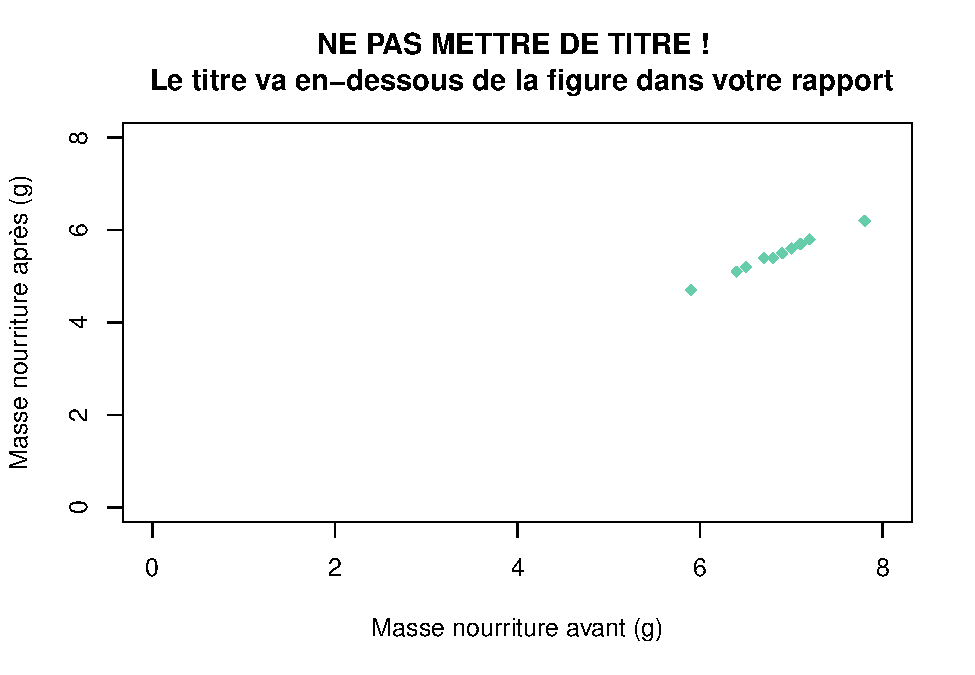
\includegraphics{Utilisation_R_base_files/figure-latex/unnamed-chunk-8-1.pdf}

\hypertarget{insuxe9rer-une-courbe-de-ruxe9gression-et-calculer-un-coefficient-de-corruxe9lation}{%
\subsubsection{3.2 - Insérer une courbe de régression (et calculer un
coefficient de
corrélation)}\label{insuxe9rer-une-courbe-de-ruxe9gression-et-calculer-un-coefficient-de-corruxe9lation}}

\hypertarget{insuxe9rer-une-courbe-de-ruxe9gression}{%
\paragraph{3.2.1 - Insérer une courbe de
régression}\label{insuxe9rer-une-courbe-de-ruxe9gression}}

Pour créer une ligne de régression qui modélise les données, il faut
créer un modèle de régression. Ici nous resterons sur les modèles
linéaires (de la forme y = ax + b).

Pour créer le modèle on utilise la fonction \texttt{lm()} (pour
\textbf{L}inear \textbf{M}odel). Sa syntaxe est la suivante:
\texttt{lm(variable\_à\_mettre\_en\_y\ \textasciitilde{}\ variable\_à\_mettre\_en\_x)}.

\begin{Shaded}
\begin{Highlighting}[]
\CommentTok{# 1/ on créé un modèle pour voir s'il peut "fitter" les données?}
\NormalTok{model <-}\StringTok{ }\KeywordTok{lm}\NormalTok{(data}\OperatorTok{$}\NormalTok{poids_sec_ap }\OperatorTok{~}\StringTok{ }\NormalTok{data}\OperatorTok{$}\NormalTok{poids_sec_av)}
\end{Highlighting}
\end{Shaded}

Une fois le modèle de régression créé, il faut regarder les propriétés
du modèle, notamment combien de variation de la variable que je cherche
à expliquer (celle qui est en y) notre modèle explique. On fait ça en
regardant la valeur du R². Le R² exprime \textbf{le pourcentage de
variation de la variable y expliqué par le modèle}. Donc plus le R² est
grand, plus le modèle explique bien la variation observée. Pour aller
chercher la valeur de R², on utilise la commande
\texttt{nom\_du\_modèle\$adj.r.squared}

On peut ensuite regarder les coefficients du modèle, c'est-à-dire la
valeur de la pente et la valeur de l'ordonnée à l'origine.

\begin{Shaded}
\begin{Highlighting}[]
\CommentTok{# 2/ on regarde les propriétés de ce modèle:}

\CommentTok{## le R² qui exprime le pourcentage de variation de y qui est expliqué par le modèle:}
\KeywordTok{summary}\NormalTok{(model)}\OperatorTok{$}\NormalTok{adj.r.squared}
\end{Highlighting}
\end{Shaded}

\begin{verbatim}
## [1] 0.9921853
\end{verbatim}

\begin{Shaded}
\begin{Highlighting}[]
\CommentTok{## les coefficients du modèle c'est à dire l'ordonnée à l'origine et la pente:}
\NormalTok{model}\OperatorTok{$}\NormalTok{coefficients}
\end{Highlighting}
\end{Shaded}

\begin{verbatim}
##       (Intercept) data$poids_sec_av 
##        -0.0243083         0.8027668
\end{verbatim}

Une fois les proriétés du modèle vérifiées, on peut afficher la droite
de régression en utilisant la fonction \texttt{abline()}. L'argument de
la fonction est tout simplement le modèle créé précédemment avec la
fonction \texttt{lm}.

\begin{Shaded}
\begin{Highlighting}[]
\CommentTok{# 3/ On peut ensuite refaire le graphique précédent en ajoutant la droite de régression }
\CommentTok{# grace à la fonction abline():}
\KeywordTok{plot}\NormalTok{(}\DataTypeTok{x =}\NormalTok{ data}\OperatorTok{$}\NormalTok{poids_sec_av, }\DataTypeTok{y =}\NormalTok{ data}\OperatorTok{$}\NormalTok{poids_sec_ap,}
     \DataTypeTok{xlim =} \KeywordTok{c}\NormalTok{(}\DecValTok{0}\NormalTok{, }\DecValTok{8}\NormalTok{), }\DataTypeTok{ylim =} \KeywordTok{c}\NormalTok{(}\DecValTok{0}\NormalTok{, }\DecValTok{8}\NormalTok{), }
     \DataTypeTok{pch =} \DecValTok{18}\NormalTok{, }
     \DataTypeTok{cex =} \DecValTok{1}\NormalTok{, }
     \DataTypeTok{col =} \StringTok{"aquamarine3"}\NormalTok{,}
     \DataTypeTok{xlab =} \StringTok{"Masse nourriture avant (g)"}\NormalTok{, }
     \DataTypeTok{ylab =} \StringTok{"Masse nourriture après (g)"}\NormalTok{,}
     \DataTypeTok{main =} \StringTok{"NE PAS METTRE DE TITRE ! }\CharTok{\textbackslash{}n}\StringTok{ Le titre va en-dessous de la figure dans votre rapport"}\NormalTok{)}
\KeywordTok{abline}\NormalTok{(model, }\DataTypeTok{col =} \StringTok{"red"}\NormalTok{)}
\end{Highlighting}
\end{Shaded}

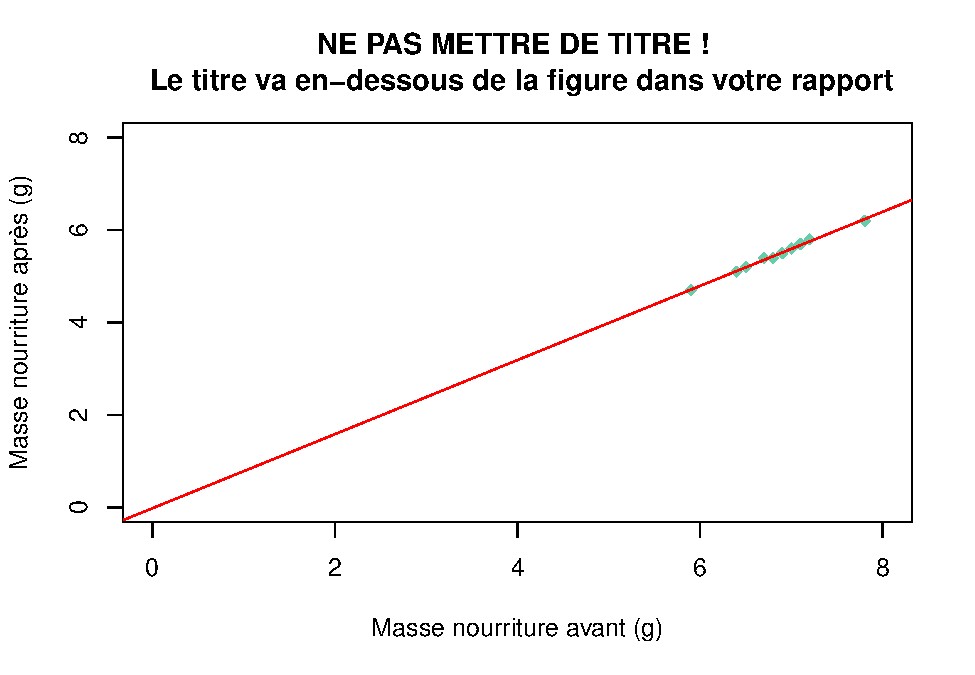
\includegraphics{Utilisation_R_base_files/figure-latex/unnamed-chunk-11-1.pdf}

\hypertarget{calculer-un-coefficient-de-corruxe9lation}{%
\paragraph{3.2.2 - Calculer un coefficient de
corrélation}\label{calculer-un-coefficient-de-corruxe9lation}}

Pour calculer le coefficient de corrélation entre deux variables, il
faut utiliser la fonction \texttt{cor()} via la syntaxe suivante :
\texttt{cor(variable\_1\ ,\ variable\_2,\ method\ =\ c("pearson"))}. Ici
on utilise un coefficient de pearson car les deux variables à étudier
sont continues.

:warning: \textbf{Correlation n'est pas causalité! } :warning:

\begin{Shaded}
\begin{Highlighting}[]
\KeywordTok{cor}\NormalTok{(data}\OperatorTok{$}\NormalTok{poids_sec_av, data}\OperatorTok{$}\NormalTok{poids_sec_ap, }\DataTypeTok{method =} \KeywordTok{c}\NormalTok{(}\StringTok{"pearson"}\NormalTok{))}
\end{Highlighting}
\end{Shaded}

\begin{verbatim}
## [1] 0.9963157
\end{verbatim}

\hypertarget{produire-un-histogramme}{%
\subsubsection{3.2 - Produire un
histogramme}\label{produire-un-histogramme}}

Pour produire un histogramme, on utilise la fonction \texttt{hist()}.
Les arguments pour le titre, la couleur et le nom des axes sont les
mêmes que ceux vus dans la partie \textbf{3.1}. Vous pouvez choisir de
représenter la fréquence d'une variable unique comme suit pour la
variable de la masse sèche avant l'expérience:

\begin{Shaded}
\begin{Highlighting}[]
\KeywordTok{hist}\NormalTok{(data}\OperatorTok{$}\NormalTok{poids_sec_av, }
     \DataTypeTok{col =} \StringTok{"aquamarine3"}\NormalTok{, }
     \DataTypeTok{main =} \StringTok{"TOUJOURS PAS DE TITRE ICI"}\NormalTok{, }
     \DataTypeTok{xlab =} \StringTok{"masses sèches (en g)"}\NormalTok{, }
     \DataTypeTok{ylab =} \StringTok{"Fréquence"}\NormalTok{)}
\end{Highlighting}
\end{Shaded}

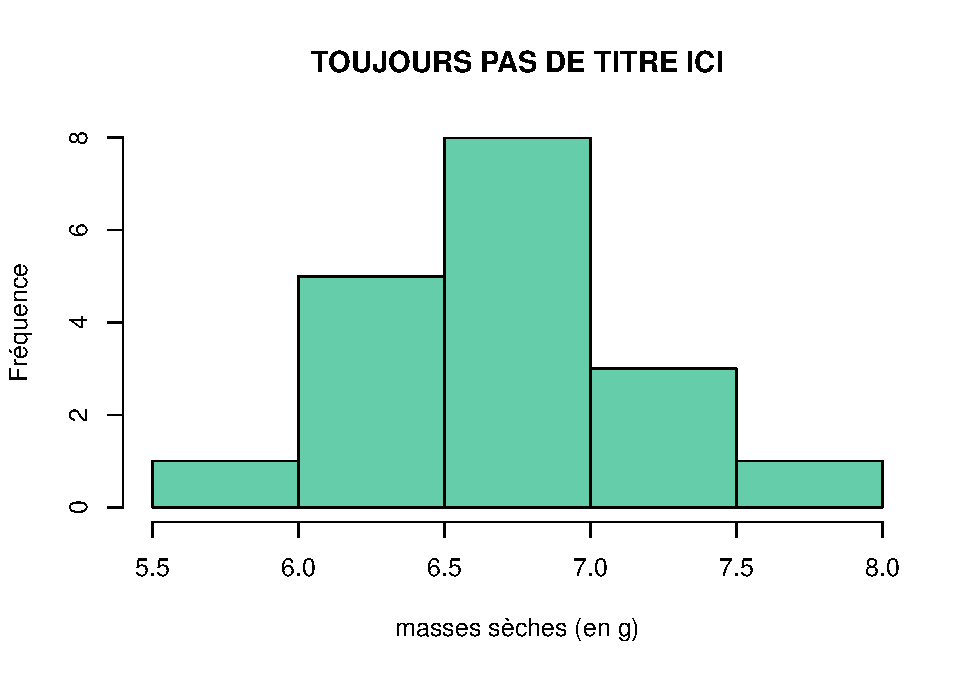
\includegraphics{Utilisation_R_base_files/figure-latex/unnamed-chunk-13-1.pdf}

\hypertarget{produire-des-bouxeetes-uxe0-moustaches}{%
\subsubsection{3.3 - Produire des boîtes à
moustaches}\label{produire-des-bouxeetes-uxe0-moustaches}}

Pour créér une boite à moustache, on utilise la fonction
\texttt{boxplot()} comme suit:
\texttt{boxplot(variable\_à\_mettre\_en\_y\ \textasciitilde{}\ variable\_à\_mettre\_en\_x)}

Les arguments pour le titre, la couleur et le nom des axes sont les
mêmes que ceux vus dans la partie \textbf{3.1}. Si on cherche à
représenter la consommation par unité de masse en fonction de l'espèce,
on code donc ainsi:

\begin{Shaded}
\begin{Highlighting}[]
\KeywordTok{boxplot}\NormalTok{(data}\OperatorTok{$}\NormalTok{conso_masse }\OperatorTok{~}\StringTok{ }\NormalTok{data}\OperatorTok{$}\NormalTok{espece, }
        \DataTypeTok{col =} \StringTok{"aquamarine3"}\NormalTok{, }
        \DataTypeTok{main =} \StringTok{"TOUJOURS PAS !!!"}\NormalTok{, }
        \DataTypeTok{xlab =} \StringTok{"espèces"}\NormalTok{, }
        \DataTypeTok{ylab =} \StringTok{"Consommation par unité de masse (g/individus)"}\NormalTok{)}
\end{Highlighting}
\end{Shaded}

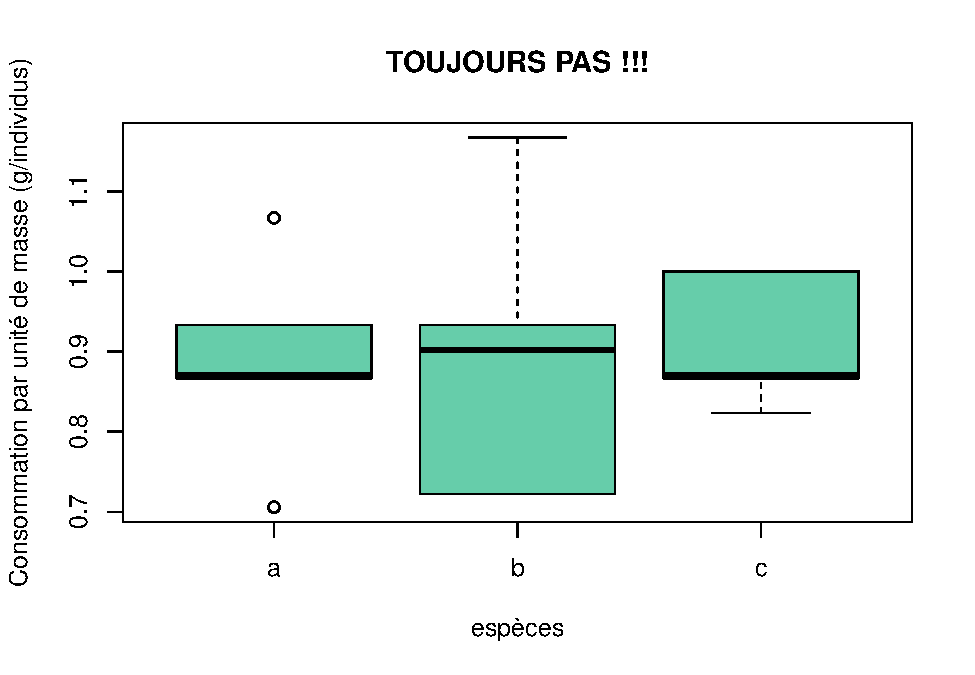
\includegraphics{Utilisation_R_base_files/figure-latex/unnamed-chunk-14-1.pdf}

Encore une fois, il est possible de faire des figures via
\texttt{ggplot2}. Vous trouverez votre bonheur ici ==\textgreater{}
:pray:\url{https://www.r-graph-gallery.com/index.html}:pray:

:tada: Voilà, vous êtes arrivés à l'étape finale des graphiques ! :tada:

\begin{figure}
\centering
\includegraphics{https://media.giphy.com/media/xT77XWum9yH7zNkFW0/giphy.gif}
\caption{Alt Text}
\end{figure}

\end{document}
